% Options for packages loaded elsewhere
\PassOptionsToPackage{unicode}{hyperref}
\PassOptionsToPackage{hyphens}{url}
%
\documentclass[
  ignorenonframetext,
  aspectratio=1610,
]{beamer}
\usepackage{pgfpages}
\setbeamertemplate{caption}[numbered]
\setbeamertemplate{caption label separator}{: }
\setbeamercolor{caption name}{fg=normal text.fg}
\beamertemplatenavigationsymbolsempty
% Prevent slide breaks in the middle of a paragraph
\widowpenalties 1 10000
\raggedbottom
\setbeamertemplate{part page}{
  \centering
  \begin{beamercolorbox}[sep=16pt,center]{part title}
    \usebeamerfont{part title}\insertpart\par
  \end{beamercolorbox}
}
\setbeamertemplate{section page}{
  \centering
  \begin{beamercolorbox}[sep=12pt,center]{part title}
    \usebeamerfont{section title}\insertsection\par
  \end{beamercolorbox}
}
\setbeamertemplate{subsection page}{
  \centering
  \begin{beamercolorbox}[sep=8pt,center]{part title}
    \usebeamerfont{subsection title}\insertsubsection\par
  \end{beamercolorbox}
}
\AtBeginPart{
  \frame{\partpage}
}
\AtBeginSection{
  \ifbibliography
  \else
    \frame{\sectionpage}
  \fi
}
\AtBeginSubsection{
  \frame{\subsectionpage}
}
\usepackage{amsmath,amssymb}
\usepackage{lmodern}
\usepackage{iftex}
\ifPDFTeX
  \usepackage[T1]{fontenc}
  \usepackage[utf8]{inputenc}
  \usepackage{textcomp} % provide euro and other symbols
\else % if luatex or xetex
  \usepackage{unicode-math}
  \defaultfontfeatures{Scale=MatchLowercase}
  \defaultfontfeatures[\rmfamily]{Ligatures=TeX,Scale=1}
\fi
% Use upquote if available, for straight quotes in verbatim environments
\IfFileExists{upquote.sty}{\usepackage{upquote}}{}
\IfFileExists{microtype.sty}{% use microtype if available
  \usepackage[]{microtype}
  \UseMicrotypeSet[protrusion]{basicmath} % disable protrusion for tt fonts
}{}
\makeatletter
\@ifundefined{KOMAClassName}{% if non-KOMA class
  \IfFileExists{parskip.sty}{%
    \usepackage{parskip}
  }{% else
    \setlength{\parindent}{0pt}
    \setlength{\parskip}{6pt plus 2pt minus 1pt}}
}{% if KOMA class
  \KOMAoptions{parskip=half}}
\makeatother
\usepackage{xcolor}
\newif\ifbibliography
\usepackage{graphicx}
\makeatletter
\def\maxwidth{\ifdim\Gin@nat@width>\linewidth\linewidth\else\Gin@nat@width\fi}
\def\maxheight{\ifdim\Gin@nat@height>\textheight\textheight\else\Gin@nat@height\fi}
\makeatother
% Scale images if necessary, so that they will not overflow the page
% margins by default, and it is still possible to overwrite the defaults
% using explicit options in \includegraphics[width, height, ...]{}
\setkeys{Gin}{width=\maxwidth,height=\maxheight,keepaspectratio}
% Set default figure placement to htbp
\makeatletter
\def\fps@figure{htbp}
\makeatother
\setlength{\emergencystretch}{3em} % prevent overfull lines
\providecommand{\tightlist}{%
  \setlength{\itemsep}{0pt}\setlength{\parskip}{0pt}}
\setcounter{secnumdepth}{-\maxdimen} % remove section numbering
\usepackage{pgfpages}
\usepackage{microtype}
\usepackage{tikz}
  \usetikzlibrary{positioning}
  \usetikzlibrary{arrows}
  \usetikzlibrary{graphs}

\definecolor{CTred}{RGB}{229,32,32}
\definecolor{CTgrey}{RGB}{153,153,153}

\usepackage{array}
\usepackage{dcolumn}
\usepackage{booktabs}

% colors: white text on 90% black background
\setbeamercolor{normal text}{fg=black,bg=white}

% light blue as a highlight color
\setbeamercolor*{structure}{fg=CTred}
\setbeamercolor{section title}{fg=CTred}
\setbeamercolor{alerted text}{use=structure,fg=CTred}
\setbeamercolor*{palette primary}{use=structure,fg=structure.fg}
\setbeamercolor*{palette secondary}{use=structure,fg=structure.fg!95!black}
\setbeamercolor*{palette tertiary}{use=structure,fg=structure.fg!90!black}
\setbeamercolor*{palette quaternary}{use=structure,fg=structure.fg!95!black,bg=black!80}

\setbeamercolor*{framesubtitle}{fg=white}


% use system fonts: here, Gill Sans
\usefonttheme{professionalfonts}
\setbeamerfont{quote}{shape=\upshape}

% eliminate silly beamer navigation line at bottom of slides
\setbeamertemplate{navigation symbols}{}

% ensure text jusfication
\usepackage{ragged2e}
\justifying

% pandoc makes 2nd-lever headers into blocks, and this ensures justification
% in blocks too
\addtobeamertemplate{block begin}{}{\justifying}




\urlstyle{same}
\usepackage[overlay,absolute]{textpos}

\setbeamertemplate{items}[square]

\TPGrid[10 mm,8 mm]{9}{8}
% beamer's left and right margin is 10 mm. The top/bottom margin is ??
% or without a header ??
% the slide dimensions are 128 mm x 96 mm
% so the resulting \TPHorizModule = 12 mm and \TPVertModule = 10 mm

% uncomment if you want biblatex for citations on slides

% \usepackage{csquotes}
% \usepackage[notes,short,noibid,backend=biber]{biblatex-chicago}
% \bibliography{course.bib} 

\providecommand{\exhibit}[2]{\includegraphics[keepaspectratio, height=0.9\textheight, width=\textwidth]{assets/img/#1}\\ {\tiny #2}}
\ifLuaTeX
  \usepackage{selnolig}  % disable illegal ligatures
\fi
\IfFileExists{bookmark.sty}{\usepackage{bookmark}}{\usepackage{hyperref}}
\IfFileExists{xurl.sty}{\usepackage{xurl}}{} % add URL line breaks if available
\urlstyle{same} % disable monospaced font for URLs
\hypersetup{
  pdftitle={When Time Really Matters: Analyzing Data in the Time of COVID},
  pdfauthor={Miklós Koren (@korenmiklos)},
  hidelinks,
  pdfcreator={LaTeX via pandoc}}

\title{When Time Really Matters: Analyzing Data in the Time of COVID}
\author{Miklós Koren (@korenmiklos)}
\date{https://economics.ceu.edu}

\begin{document}
\frame{\titlepage}

\hypertarget{introduction}{%
\section{Introduction}\label{introduction}}

\begin{frame}{My first investment into econometrics}
\protect\hypertarget{my-first-investment-into-econometrics}{}
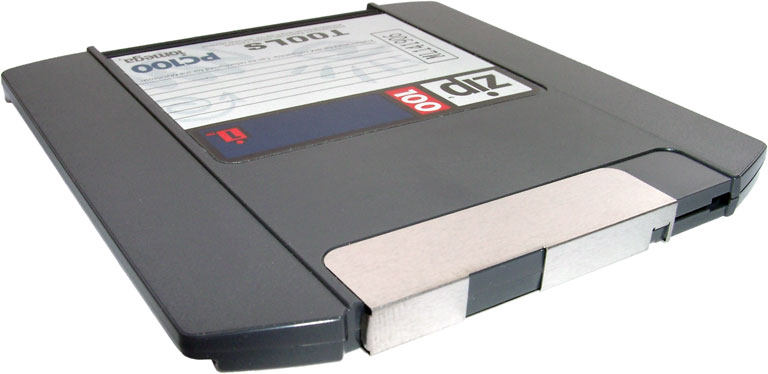
\includegraphics{exhibit/zipdrive.jpg}
\end{frame}

\begin{frame}[fragile]{My tools}
\protect\hypertarget{my-tools}{}
\begin{verbatim}
economics,1994-
econometrics,1996-
stata,1997-
python,2003-
julia,2017-
\end{verbatim}
\end{frame}

\begin{frame}{Outline}
\protect\hypertarget{outline}{}
\begin{enumerate}
\tightlist
\item
  When time really matters
\item
  Examples of real-time data
\item
  Challenges of private data
\item
  What can economists do?
\end{enumerate}
\end{frame}

\hypertarget{when-time-really-matters}{%
\section{When time really matters}\label{when-time-really-matters}}

\begin{frame}{When time really matters}
\protect\hypertarget{when-time-really-matters-1}{}
\begin{itemize}
\tightlist
\item
  November 2019: outbreak in Wuhan
\item
  December 27, 2019: new coronarivus
\item
  December 31, 2019: WHO informed
\item
  January 30, 2020: WHO declares ``public health emergency'\,'
\item
  March 11, 2020: WHO declares pandemic
\item
  by March 31, 2020: most countries adopted strict social distancing
  measures
\end{itemize}
\end{frame}

\begin{frame}{Typical statistics publication calendar (BLS.gov)}
\protect\hypertarget{typical-statistics-publication-calendar-bls.gov}{}
\begin{figure}
\centering
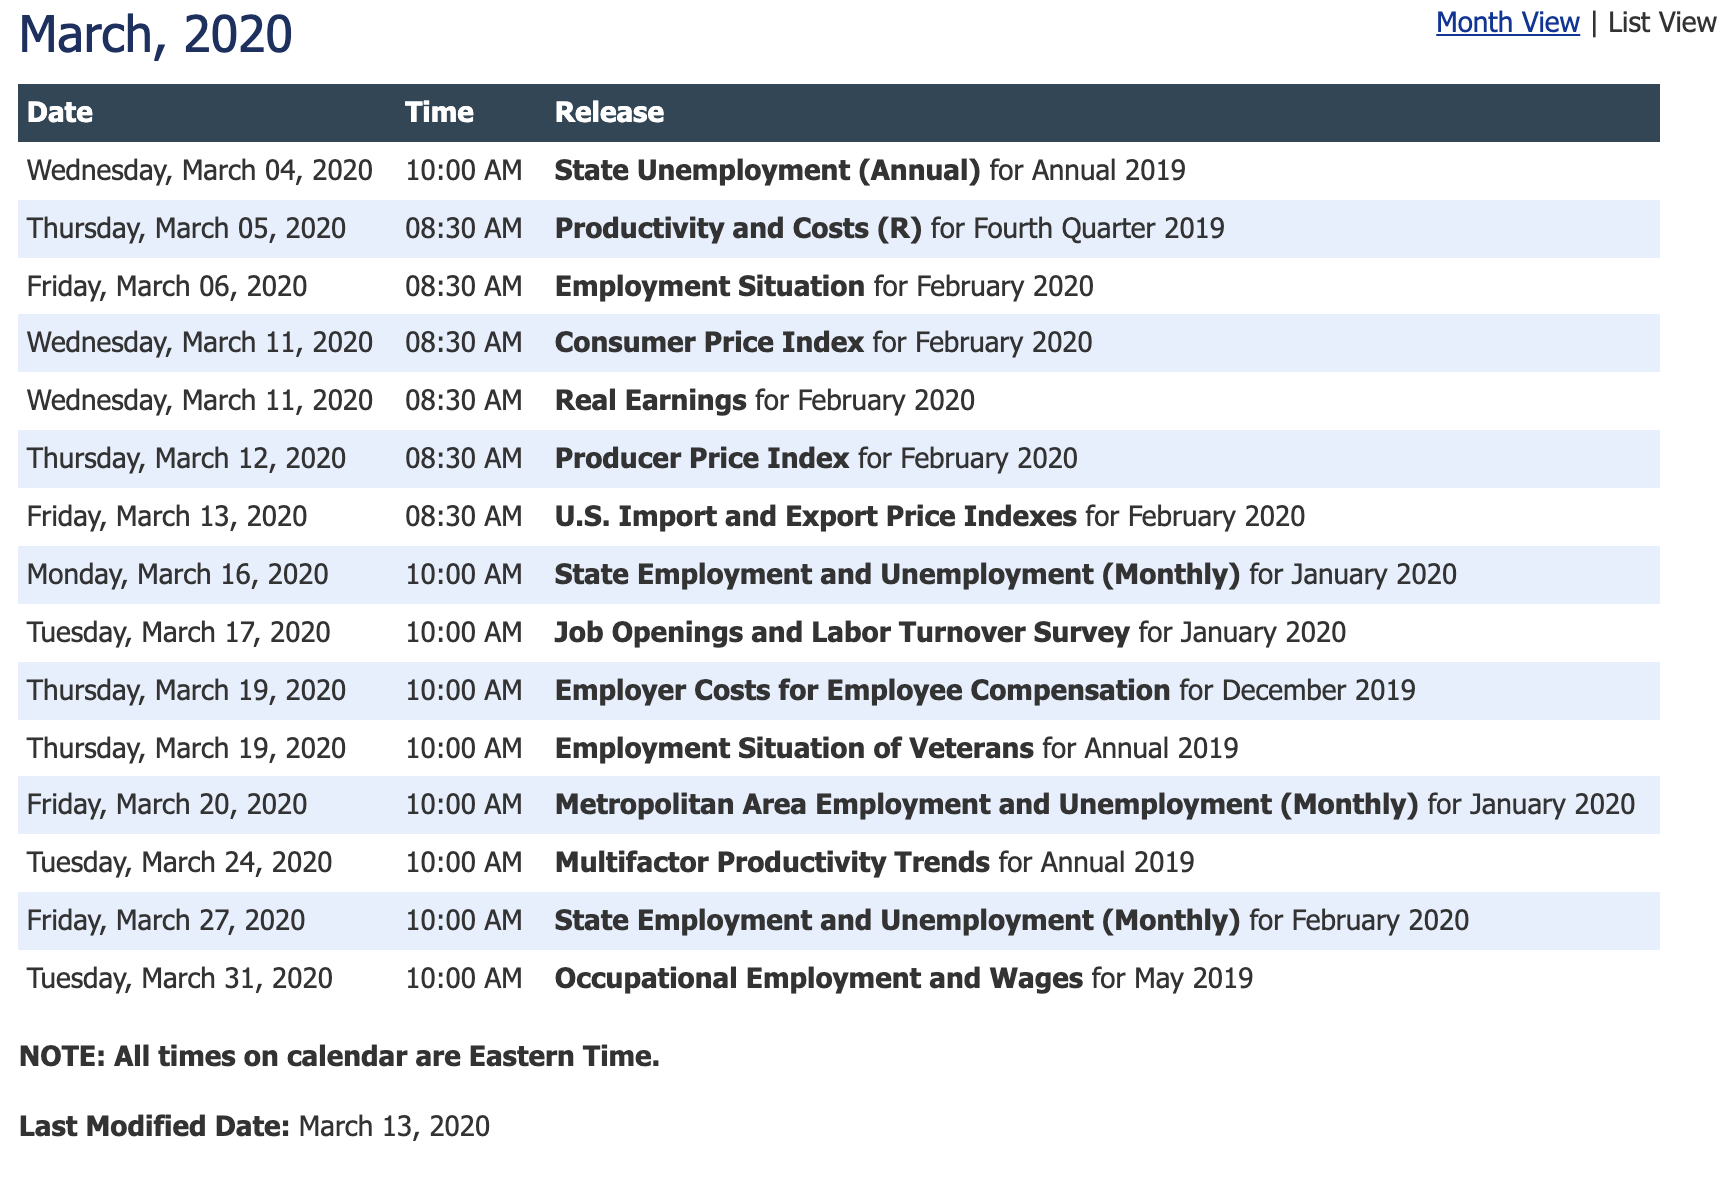
\includegraphics{exhibit/fig/bls-march-2020.png}
\caption{BLS 2020}
\end{figure}
\end{frame}

\begin{frame}{Time-sensitive questions}
\protect\hypertarget{time-sensitive-questions}{}
\begin{itemize}
\tightlist
\item
  How does the virus spread?
\item
  How many ventilators, PPEs, nurses etc. will we need? By when?
\item
  What (non-pharmaceutical) interventions are effective against it?
\item
  Which of these are most cost effective?
\item
  What can policy do to mitigate the costs?
\item
  (in addition to genome sequencing, drug and vaccine development,
  clinical research)
\end{itemize}
\end{frame}

\hypertarget{the-response-of-open-science}{%
\section{The response of open
science}\label{the-response-of-open-science}}

\begin{frame}{The response of open science}
\protect\hypertarget{the-response-of-open-science-1}{}
\begin{itemize}
\tightlist
\item
  Government, academia and industry came together quickly and
  effectively. (But: pressing issues remain.)
\item
  Troves of data shared.
\item
  Research results published fast.

  \begin{itemize}
  \tightlist
  \item
    83 issues of \emph{Covid Economics}, about 500 papers published.
  \end{itemize}
\end{itemize}

\begin{block}{Is this the future of policy analysis?}
\protect\hypertarget{is-this-the-future-of-policy-analysis}{}
\end{block}
\end{frame}

\begin{frame}{About 250,000 Covid-related articles}
\protect\hypertarget{about-250000-covid-related-articles}{}
\begin{figure}
\centering

\includegraphics{exhibit/fig/google-scholar.png}
\caption{Google Scholar 2021}
\end{figure}
\end{frame}

\begin{frame}{Our model-informed prediction based on past data (Koren
and Pető 2020)}
\protect\hypertarget{our-model-informed-prediction-based-on-past-data-koren-and-petux151-2020}{}
https://datawrapper.dwcdn.net/NNmIa/2/
\end{frame}

\begin{frame}{\ldots turned out to be quite accurate}
\protect\hypertarget{turned-out-to-be-quite-accurate}{}
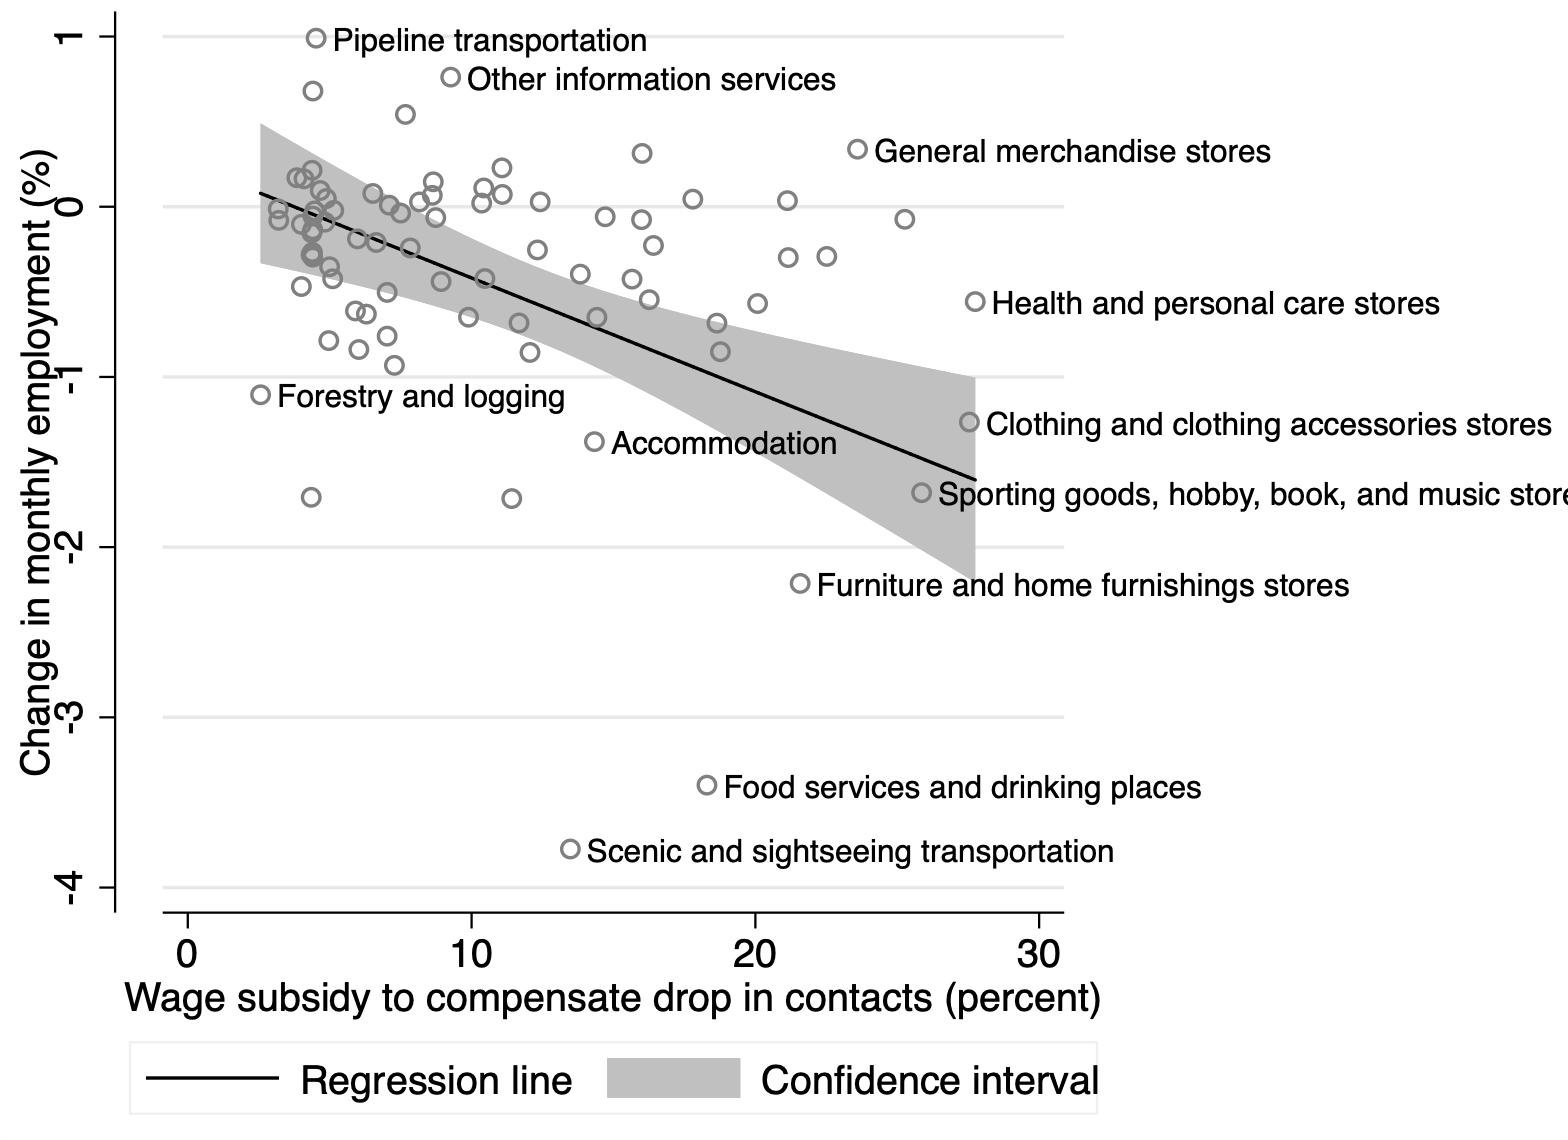
\includegraphics{exhibit/fig5.png}
\end{frame}

\begin{frame}{Timely data collection}
\protect\hypertarget{timely-data-collection}{}
How to avoid the 2-3-month lag of official statistical releases? (Plus
several months of peer review.)

Reuse existing data collected during ``normal course of business'\,':

\begin{itemize}
\tightlist
\item
  administrative
\item
  private
\end{itemize}
\end{frame}

\hypertarget{examples-of-real-time-data}{%
\section{Examples of real-time data}\label{examples-of-real-time-data}}

\begin{frame}{Visits to retail and recreation places collapsed}
\protect\hypertarget{visits-to-retail-and-recreation-places-collapsed}{}
\begin{figure}
\centering
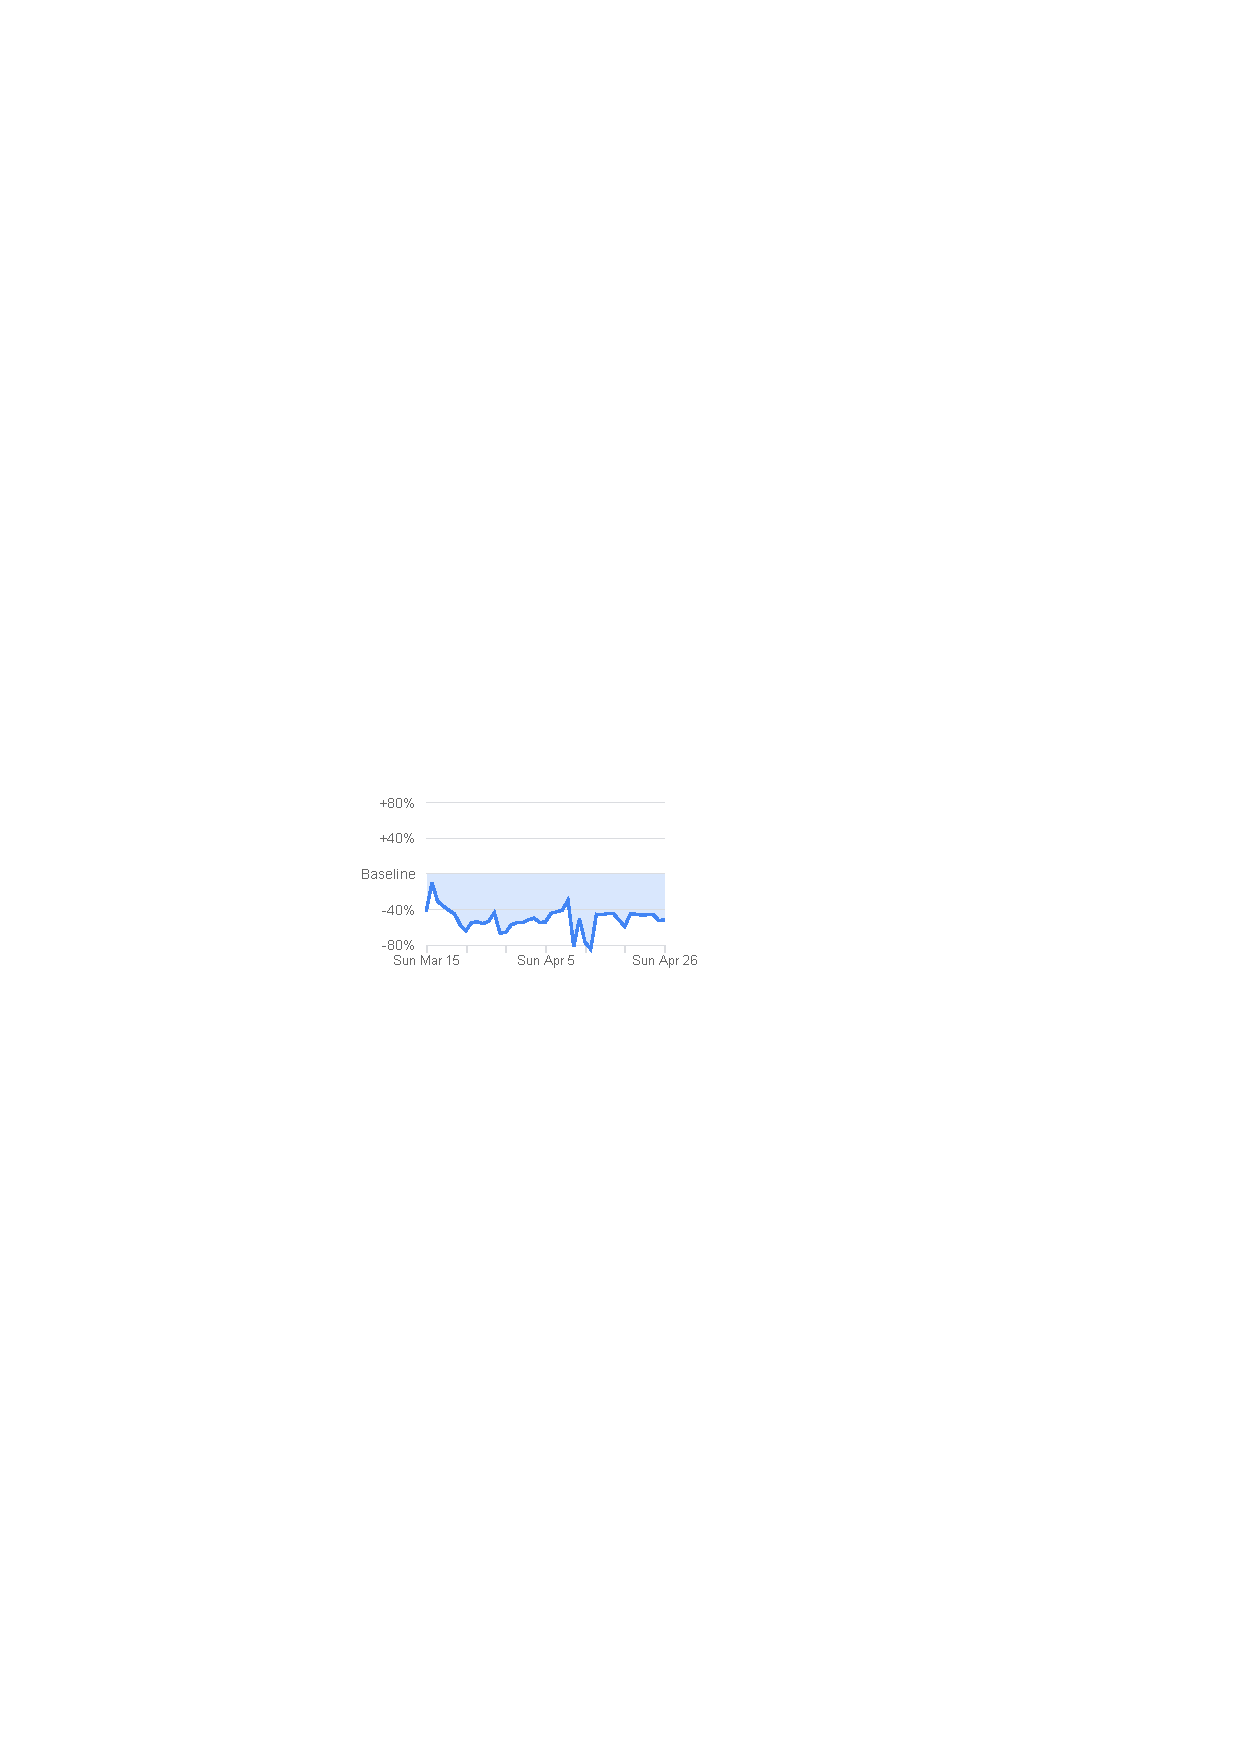
\includegraphics[width=1\textwidth,height=\textheight]{exhibit/fig/gmr-retail.pdf}
\caption{Data from Hungarian cell phone users (Google Mobility Report
2020)}
\end{figure}
\end{frame}

\begin{frame}{Many workplaces are shuttered}
\protect\hypertarget{many-workplaces-are-shuttered}{}
\begin{figure}
\centering
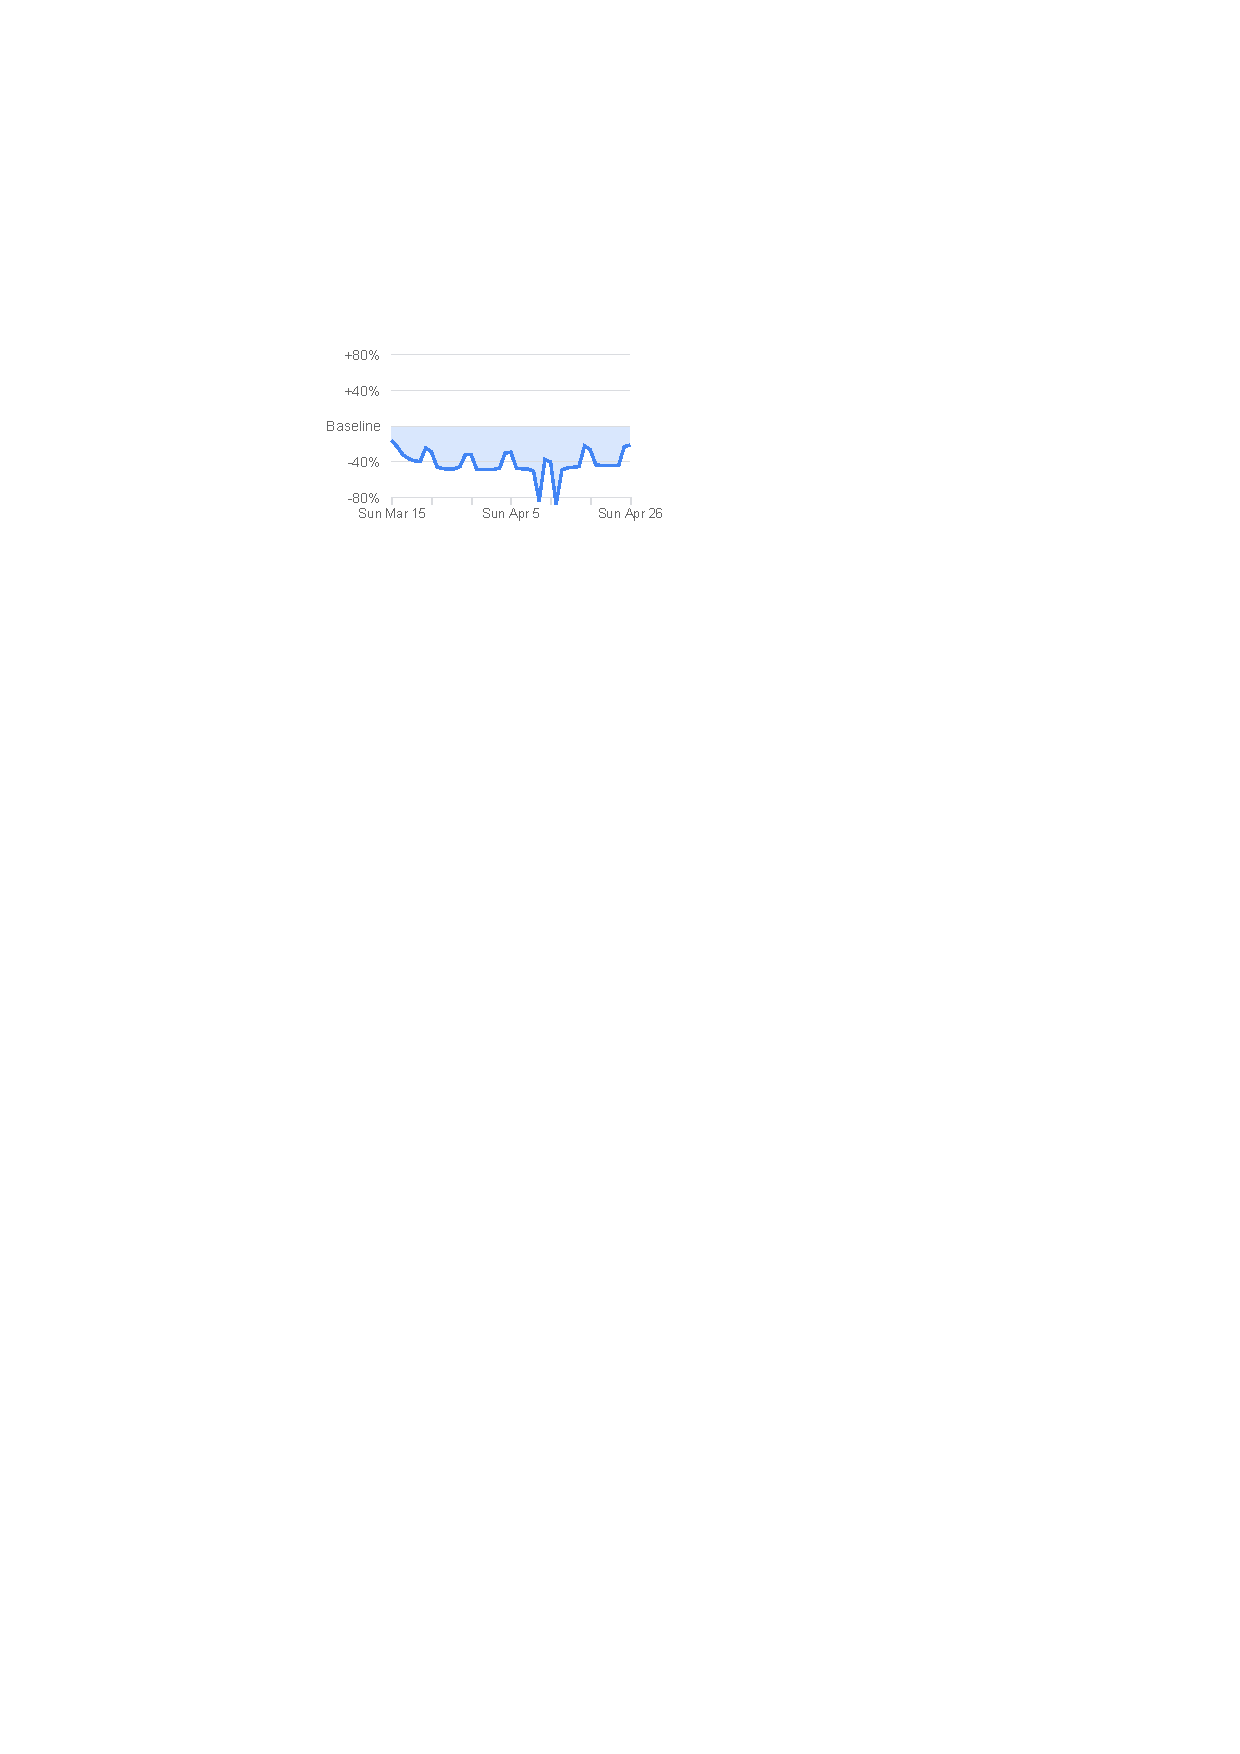
\includegraphics[width=1\textwidth,height=\textheight]{exhibit/fig/gmr-work.pdf}
\caption{Data from Hungarian cell phone users (Google Mobility Report
2020)}
\end{figure}
\end{frame}

\begin{frame}{People are staying at home}
\protect\hypertarget{people-are-staying-at-home}{}
\begin{figure}
\centering
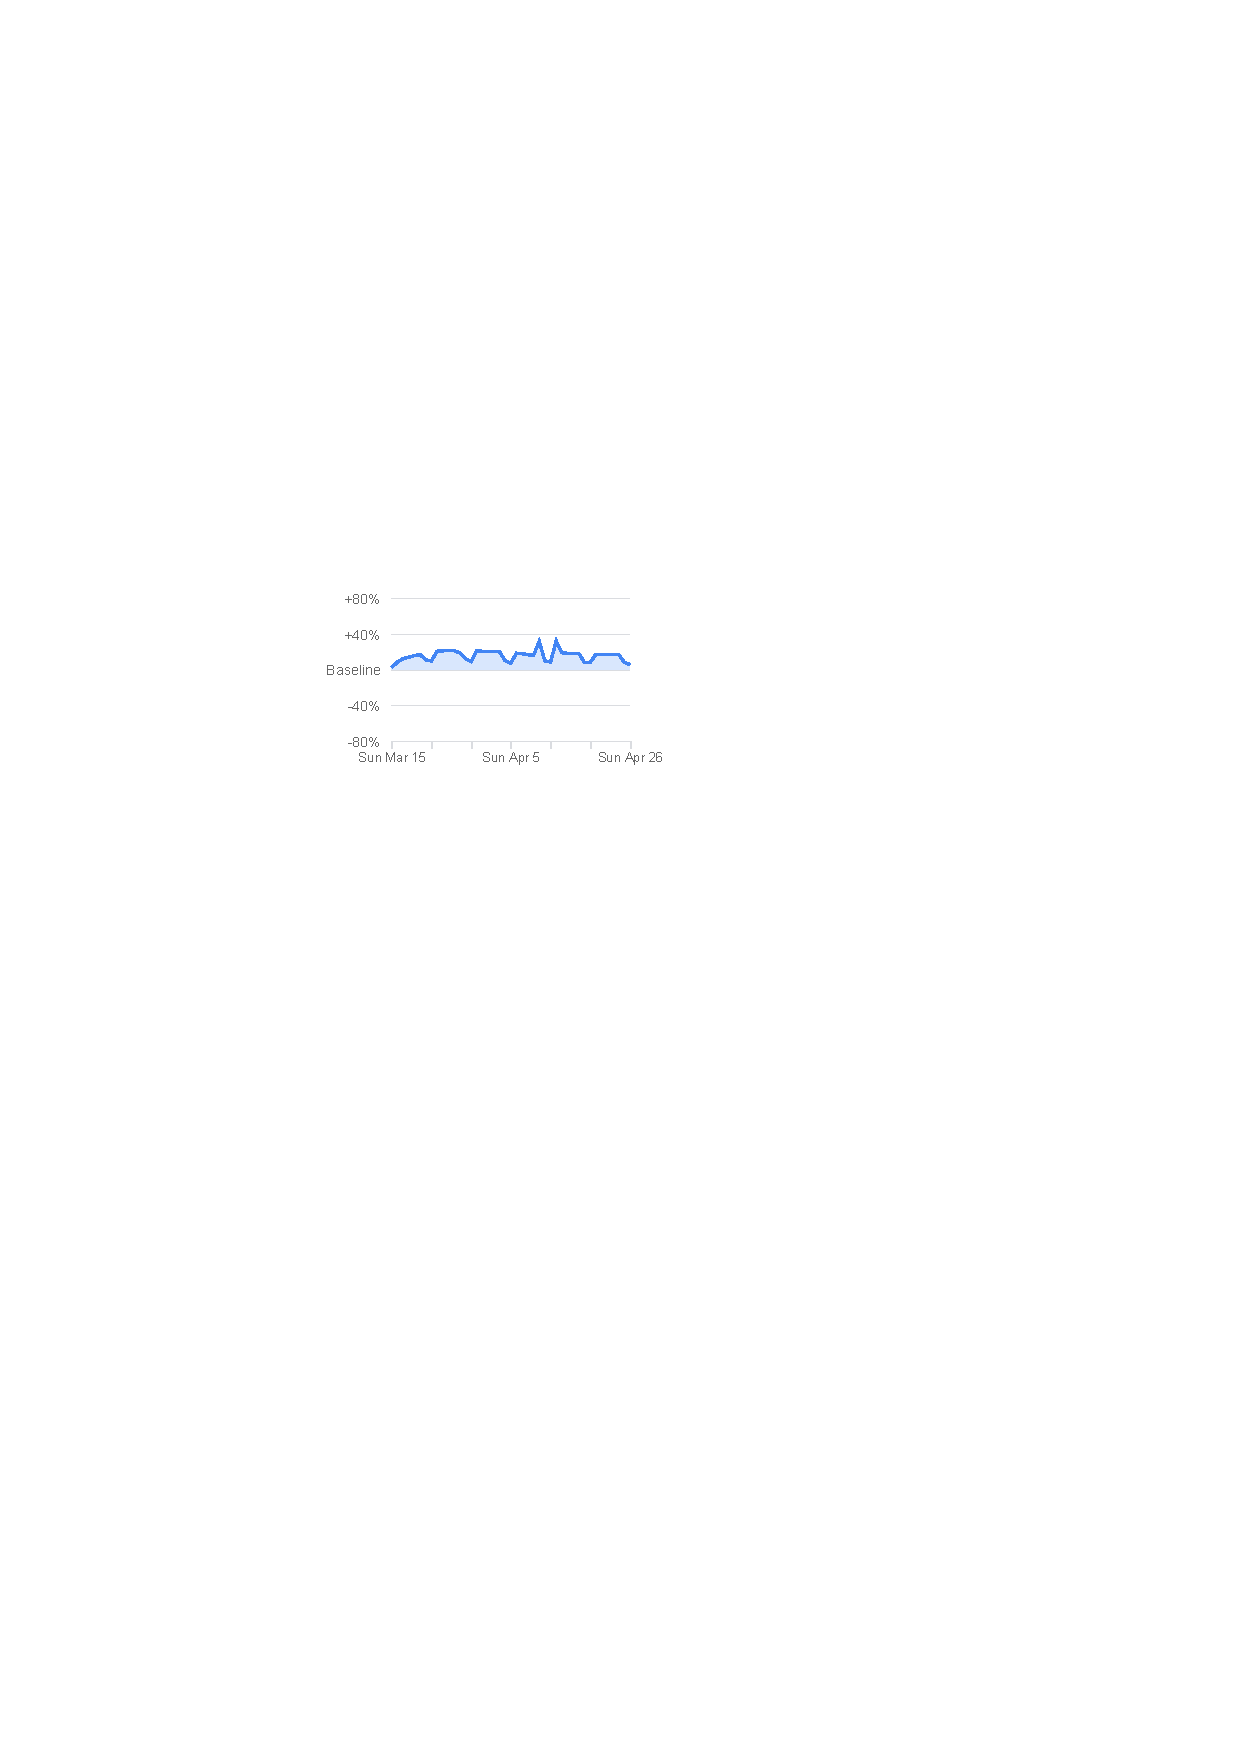
\includegraphics[width=1\textwidth,height=\textheight]{exhibit/fig/gmr-home.pdf}
\caption{Data from Hungarian cell phone users (Google Mobility Report
2020)}
\end{figure}
\end{frame}

\begin{frame}{Examples of real-time data (1)}
\protect\hypertarget{examples-of-real-time-data-1}{}
\begin{block}{Medical}
\protect\hypertarget{medical}{}
Enormous amount of clinical, epi, virology data sharing
\end{block}

\begin{block}{Stock returns}
\protect\hypertarget{stock-returns}{}
Stock prices react to news almost instantaneously. But: noisy, only for
traded stocks.
\end{block}

\begin{block}{Financial transactions}
\protect\hypertarget{financial-transactions}{}
Credit cards. Bank transactions.
\end{block}
\end{frame}

\begin{frame}{Examples of real-time data (2)}
\protect\hypertarget{examples-of-real-time-data-2}{}
\begin{block}{Tracking mobility, spatial effects}
\protect\hypertarget{tracking-mobility-spatial-effects}{}
Cell phone tracking. Visiting POIs. Contact tracing. Air travel. Real
estate pricing.
\end{block}

\begin{block}{Economic activity on platforms}
\protect\hypertarget{economic-activity-on-platforms}{}
Restaurant closures (Yelp). Ride sharing. Airbnb. Online work.
E-commerce.
\end{block}
\end{frame}

\begin{frame}{Other data sources}
\protect\hypertarget{other-data-sources}{}
\begin{block}{Other data to track infections}
\protect\hypertarget{other-data-to-track-infections}{}
Virus concentration in sewage.
\end{block}

\begin{block}{Other data to track the economy}
\protect\hypertarget{other-data-to-track-the-economy}{}
Electricity consumption. Job ads. Trademark applications.
\end{block}

\begin{block}{Other data to track social outcomes}
\protect\hypertarget{other-data-to-track-social-outcomes}{}
Religiousity. Schools and learning. Fertility. Nostalgia.
\end{block}
\end{frame}

\hypertarget{challenges-of-private-data}{%
\section{Challenges of private data}\label{challenges-of-private-data}}

\begin{frame}{Challenges of private data}
\protect\hypertarget{challenges-of-private-data-1}{}
\begin{enumerate}
\tightlist
\item
  Statistics
\item
  Accountability
\end{enumerate}
\end{frame}

\hypertarget{statistics}{%
\section{Statistics}\label{statistics}}

\begin{frame}{Data Science}
\protect\hypertarget{data-science}{}
``procedures for analyzing data, techniques for interpreting the results
of such procedures, ways of planning the gathering of data to make its
analysis easier, more precise or more accurate, and all the machinery
and results of (mathematical) statistics which apply to analyzing
data.'' (Tukey, \uncover<2>{1962})
\end{frame}

\begin{frame}{Why statistics matters}
\protect\hypertarget{why-statistics-matters}{}
Statistics provides rules for generalizing from (limited) data.
\end{frame}

\begin{frame}{A short history of (frequentist) statistics (Salsburg
2002)}
\protect\hypertarget{a-short-history-of-frequentist-statistics-salsburg-2002}{}
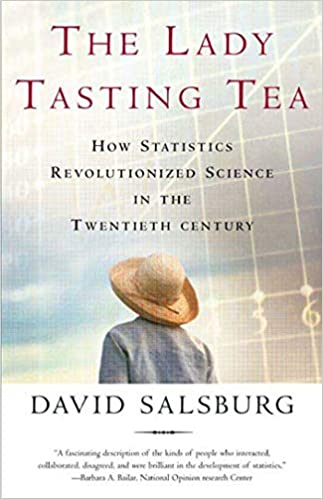
\includegraphics{exhibit/lady-tasting-tea.jpg}
\end{frame}

\begin{frame}{The evolution of statistics (Efron and Hastie)}
\protect\hypertarget{the-evolution-of-statistics-efron-and-hastie}{}
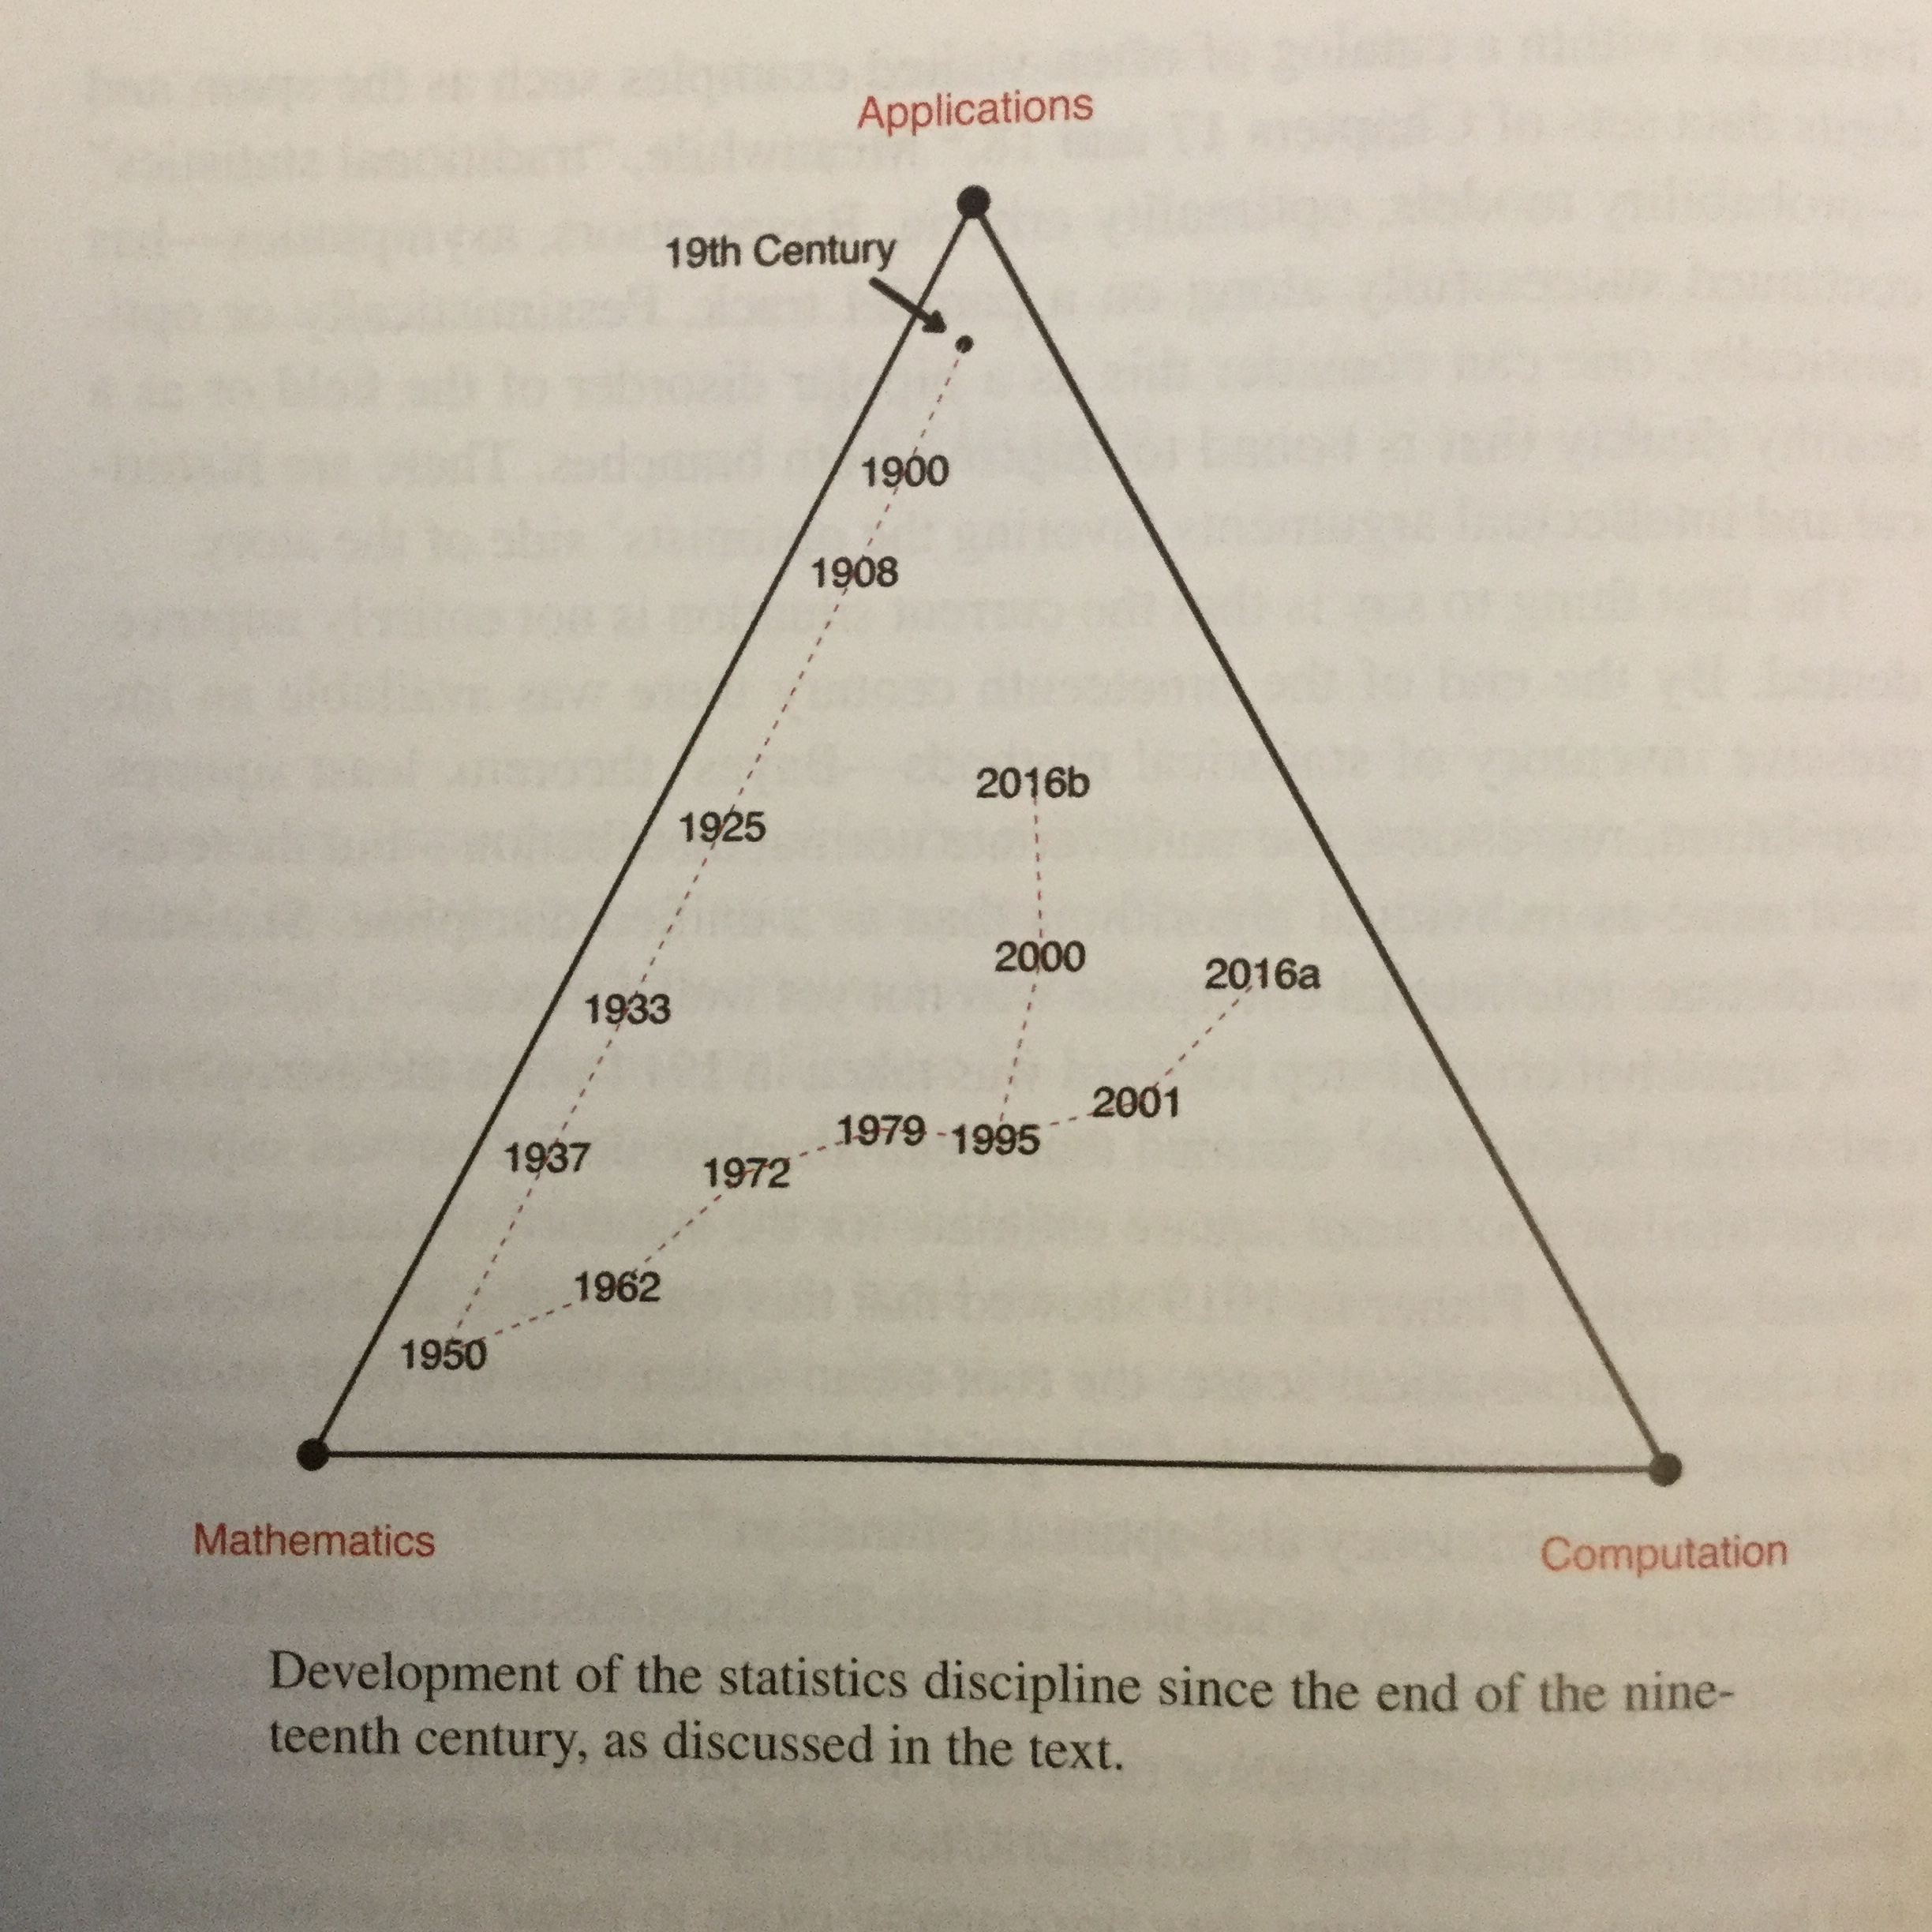
\includegraphics{exhibit/efron-hastie.jpg}
\end{frame}

\begin{frame}{Stories vs statistics}
\protect\hypertarget{stories-vs-statistics}{}
Suppose you want to predict the outcome of U.S. presidential elections
in Pennsylvania. What are the benefits of a statistical prediction
relative to talking to friends and watching TV pundits?

\begin{enumerate}
\tightlist
\item
  \(n=1\) vs \(n=\text{many}\). (``The plural of anecdote is data.'\,'
  /Raymond Wolfinger)
\item
  Stories subject to biases.
\item
  Biases are unknown and hard to account for.
\end{enumerate}
\end{frame}

\begin{frame}{Sample vs population}
\protect\hypertarget{sample-vs-population}{}
Suppose you ask 1,000 Pennsylvania voters. \[
\hat p = \frac {\# \text{Republican}}{1000}
\] \[
\text{s.e.}(\hat p) = \sqrt{\frac {\hat p (1-\hat p)}{1000}} \approx 0.016
\] if \(\hat p\approx 0.5\).
\end{frame}

\begin{frame}{Rules of generalizing from sample}
\protect\hypertarget{rules-of-generalizing-from-sample}{}
Suppose

\begin{enumerate}
\tightlist
\item
  random
\item
  independent sample
\item
  full compliance.
\end{enumerate}

(1+3 ensure representativity, 2 dictates statistical properties)

\begin{itemize}
\tightlist
\item
  Then estimation accuracy increases with \(\sqrt{n}\).
\item
  Irrespective of size of population.
\end{itemize}
\end{frame}

\hypertarget{selection-bias}{%
\section{Selection bias}\label{selection-bias}}

\begin{frame}{Selection bias}
\protect\hypertarget{selection-bias-1}{}
If sample is not representative, may suffer from \textbf{selection
bias}.

\begin{enumerate}
\tightlist
\item
  nonrandom selection into sample
\item
  nonrandom response rate
\end{enumerate}
\end{frame}

\begin{frame}{Getting a representative sample}
\protect\hypertarget{getting-a-representative-sample}{}
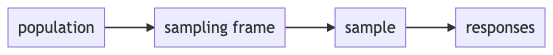
\includegraphics{exhibit/fig/selection-bias.png}

Selection may occur at each of these steps.

\begin{itemize}
\tightlist
\item
  phone survey not representative
\item
  people do not respond
\item
  some voters hide their preferences
\end{itemize}
\end{frame}

\begin{frame}{Sample vs big data}
\protect\hypertarget{sample-vs-big-data}{}
Selection bias surely does not matter if we observe (almost) everyone?!
\end{frame}

\begin{frame}{Electoral forecasts}
\protect\hypertarget{electoral-forecasts}{}
\begin{itemize}
\tightlist
\item
  based on random sample
\item
  based on votes already counted
\end{itemize}

Both are helpful but have very different properties.
\end{frame}

\begin{frame}{The blue shift}
\protect\hypertarget{the-blue-shift}{}
\begin{figure}
\centering
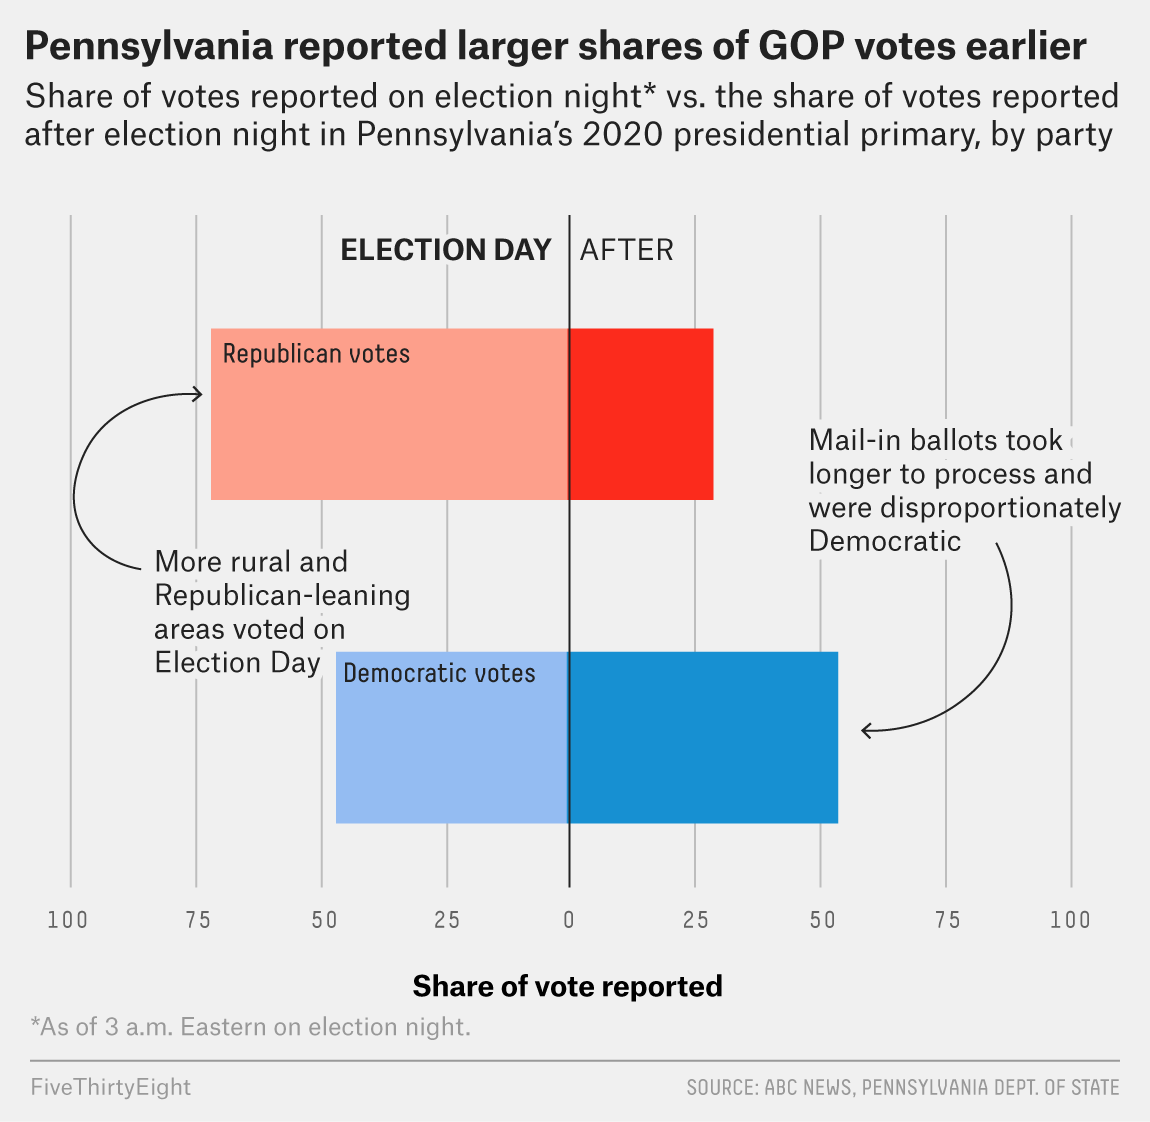
\includegraphics[width=\textwidth,height=0.8\textheight]{exhibit/fig/blue-shift.png}
\caption{FiveThirtyEight 2020}
\end{figure}
\end{frame}

\begin{frame}{Lessons from statistics}
\protect\hypertarget{lessons-from-statistics}{}
\begin{quote}
\textbf{It is better to have a small unbiased sample than a large biased
one.}
\end{quote}

Can you think of sources of selection bias in private data?
\end{frame}

\hypertarget{accountability}{%
\section{Accountability}\label{accountability}}

\begin{frame}{Accountability}
\protect\hypertarget{accountability-1}{}
\begin{enumerate}
\tightlist
\item
  Conflict of interest to share information

  \begin{itemize}
  \tightlist
  \item
    governments
  \item
    corporations
  \end{itemize}
\item
  Privacy and surveillance
\end{enumerate}
\end{frame}

\begin{frame}{Uber uses data and economists as PR props}
\protect\hypertarget{uber-uses-data-and-economists-as-pr-props}{}
``Ride-hailing apps have created jobs for Paris's poorer youth, but a
regulatory clampdown looms,'' the {[}FT{]} article said. Thesmar was
quoted in the piece saying that Uber was a ``social gamechanger''.

``We see low risk here because we can work with Landier on framing the
study and we also decide what data we share with him.'' (senior Uber
staffer quoted in Lawrence 2022)
\end{frame}

\begin{frame}{Is ride sharing killing people?}
\protect\hypertarget{is-ride-sharing-killing-people}{}
Barrios, Hochberg and Yi (2018): Uber and Lyft increased traffic and
congestion. Associated with 2--3\% increase in fatalities.

Got no data from Uber!
\end{frame}

\begin{frame}{A case study in accountability}
\protect\hypertarget{a-case-study-in-accountability}{}
Simonsohn, Simmons, Nelson and anonymous (2021) show that Shu, Mazar,
Gino, Ariely and Bazerman (2012 PNAS) is based on \textbf{fraudulent}
data.

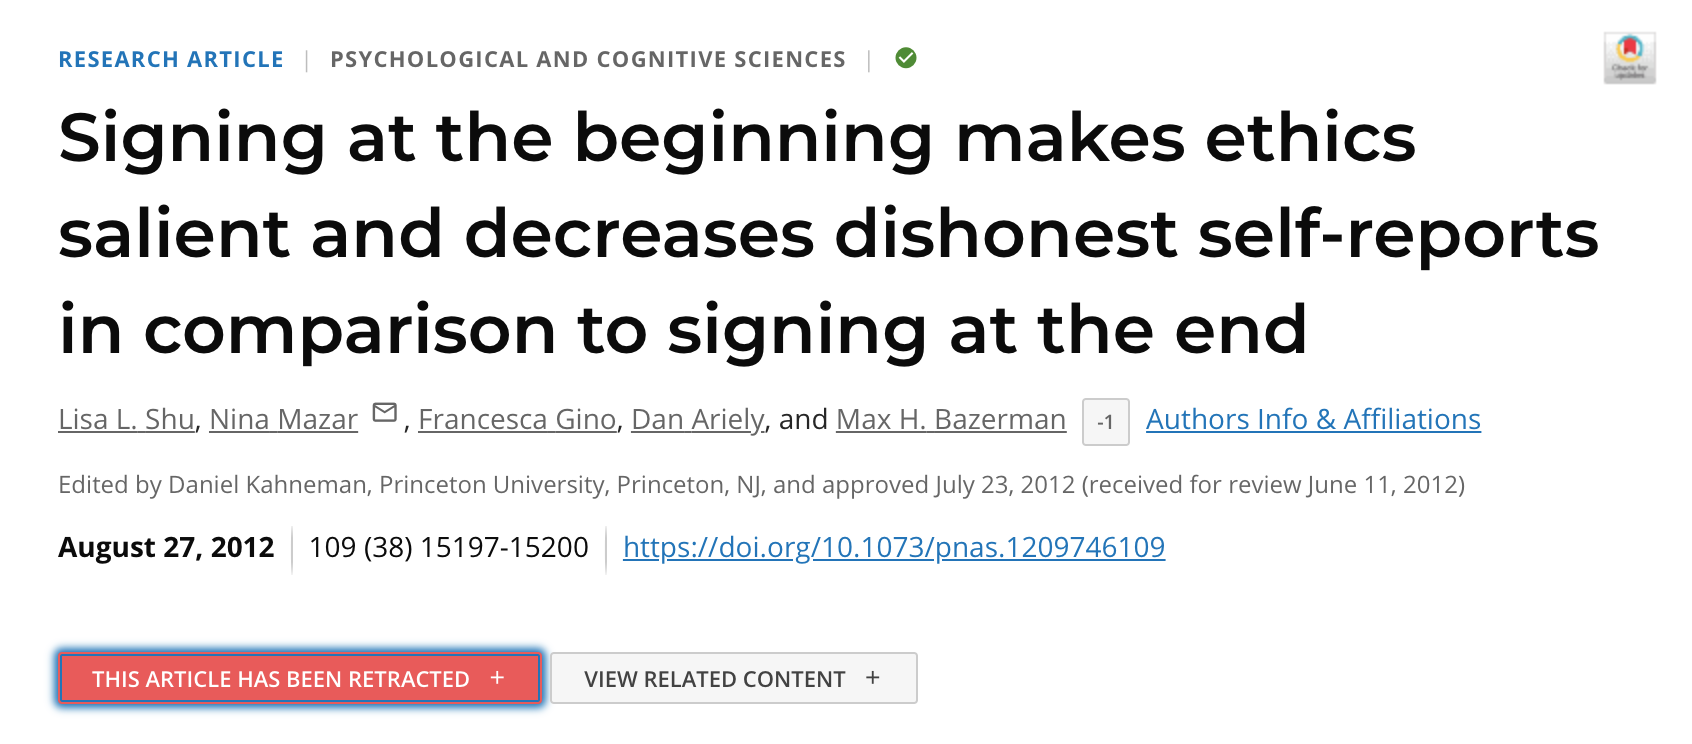
\includegraphics{exhibit/ariely.png}
\end{frame}

\begin{frame}{The data as (purportedly) shared with the private company}
\protect\hypertarget{the-data-as-purportedly-shared-with-the-private-company}{}
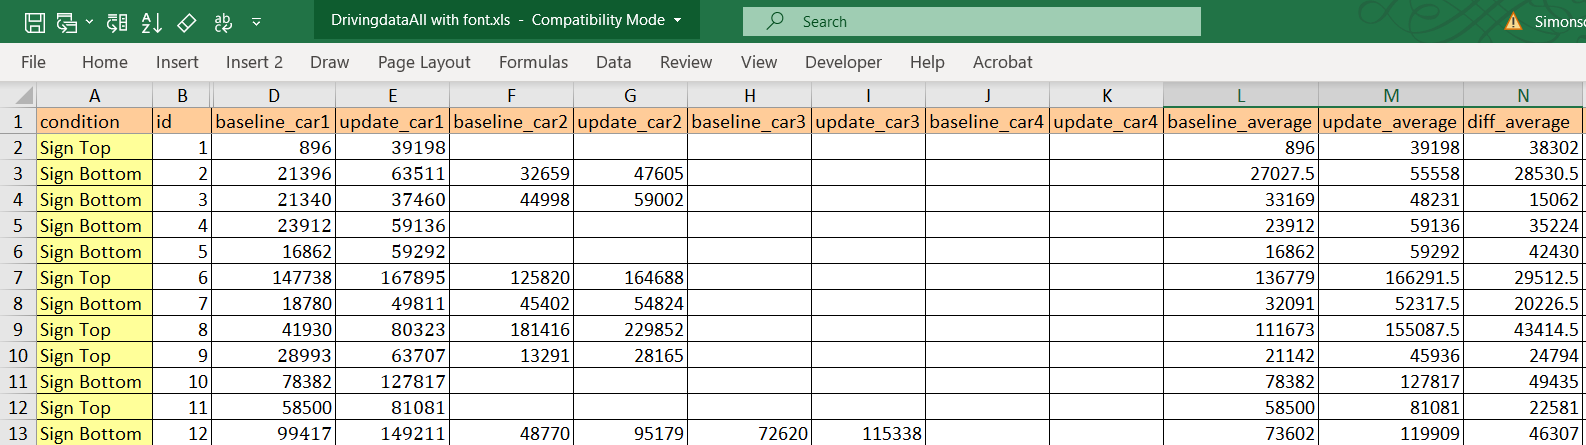
\includegraphics{exhibit/1-First-introduction-to-data.png}
\end{frame}

\begin{frame}{Distribution of miles driven in a year}
\protect\hypertarget{distribution-of-miles-driven-in-a-year}{}
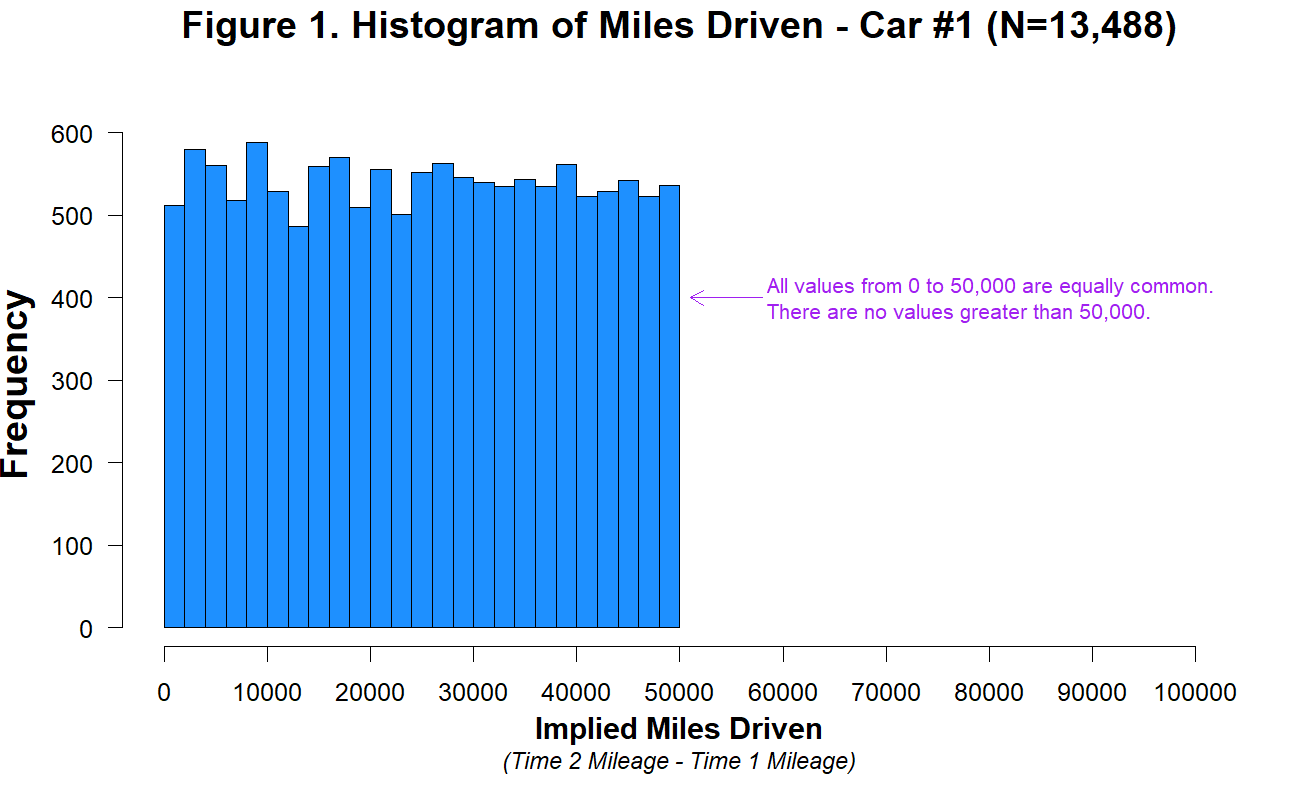
\includegraphics{exhibit/F1-Uniform-change-2021-07-03.png}
\end{frame}

\begin{frame}{No rounding in end-of-year reported mileage}
\protect\hypertarget{no-rounding-in-end-of-year-reported-mileage}{}
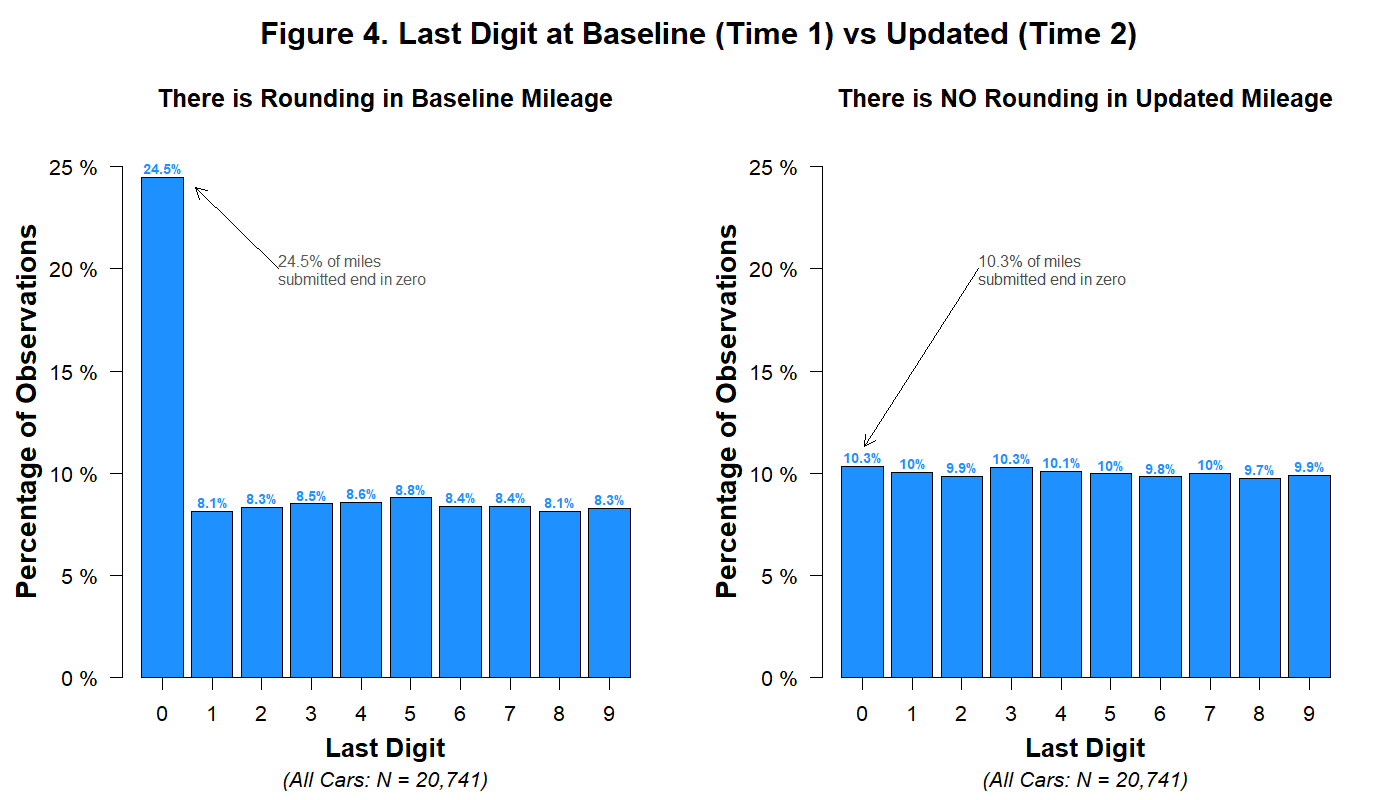
\includegraphics{exhibit/F4-Last-1-digit-2021-07-05.png}
\end{frame}

\begin{frame}{Most observations seem to be duplicated}
\protect\hypertarget{most-observations-seem-to-be-duplicated}{}
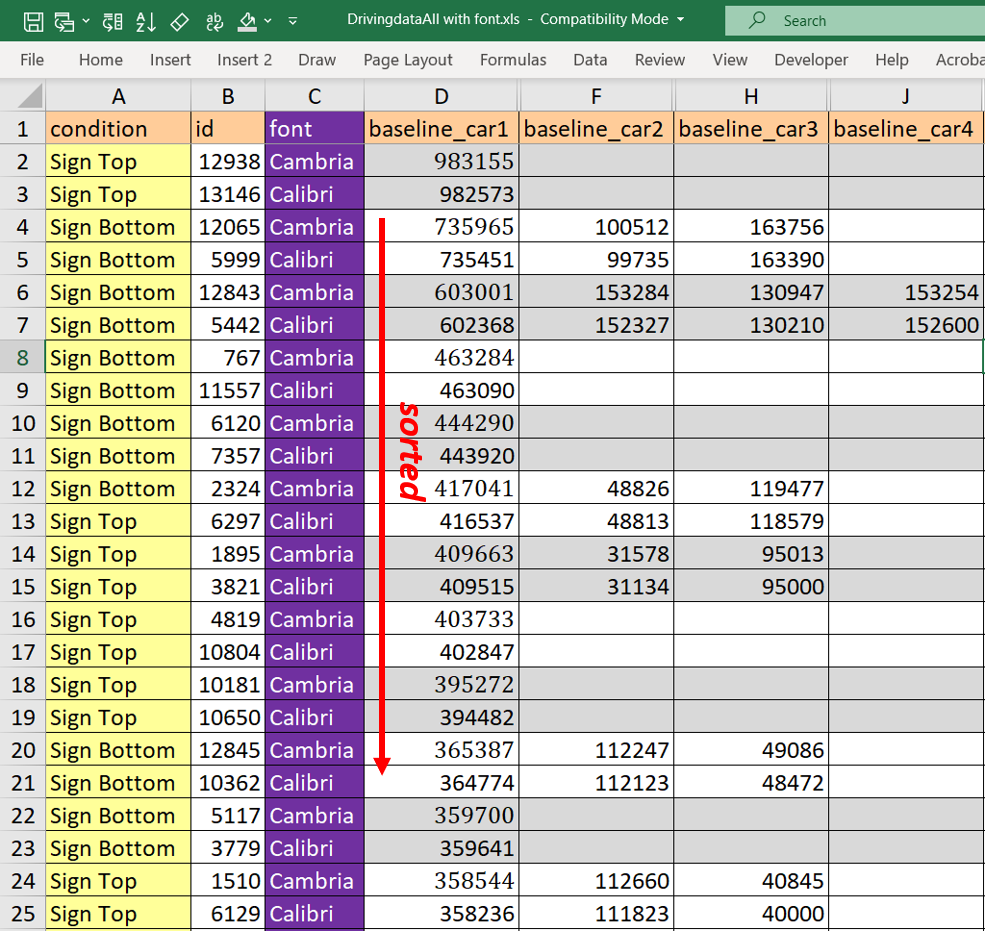
\includegraphics{exhibit/3-sort-by-car-4-2021-07-07.png}
\end{frame}

\begin{frame}{The chain of data provenance}
\protect\hypertarget{the-chain-of-data-provenance}{}
insurance company \(\to\) Ariely \(\to\) Mazar \(\to\) PNAS
\end{frame}

\hypertarget{what-can-economists-do}{%
\section{What can economists do?}\label{what-can-economists-do}}

\begin{frame}{What can economists do?}
\protect\hypertarget{what-can-economists-do-1}{}
Three tenets of economics:

\begin{enumerate}
\tightlist
\item
  People respond to incentives.
\item
  Systems matter.
\item
  Scarce resources are worth more.
\end{enumerate}
\end{frame}

\begin{frame}{The Susceptible-Infectious-Recovered model}
\protect\hypertarget{the-susceptible-infectious-recovered-model}{}
\begin{figure}
\centering
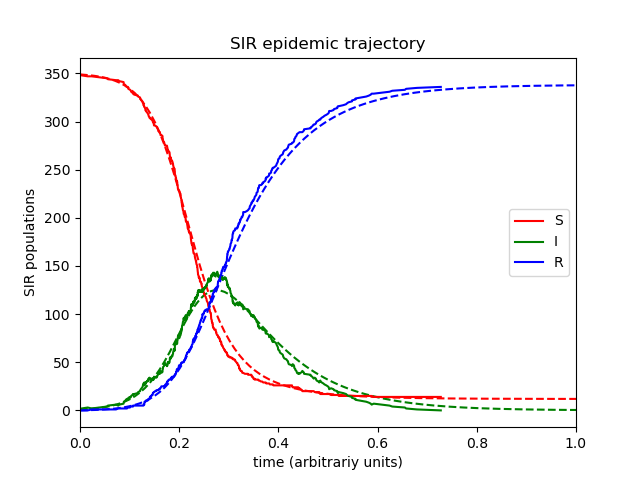
\includegraphics[width=\textwidth,height=0.8\textheight]{exhibit/fig/SIR_trajectory.png}
\caption{Wefatherley 2018}
\end{figure}
\end{frame}

\begin{frame}{Flattening the curve}
\protect\hypertarget{flattening-the-curve}{}
\begin{figure}
\centering
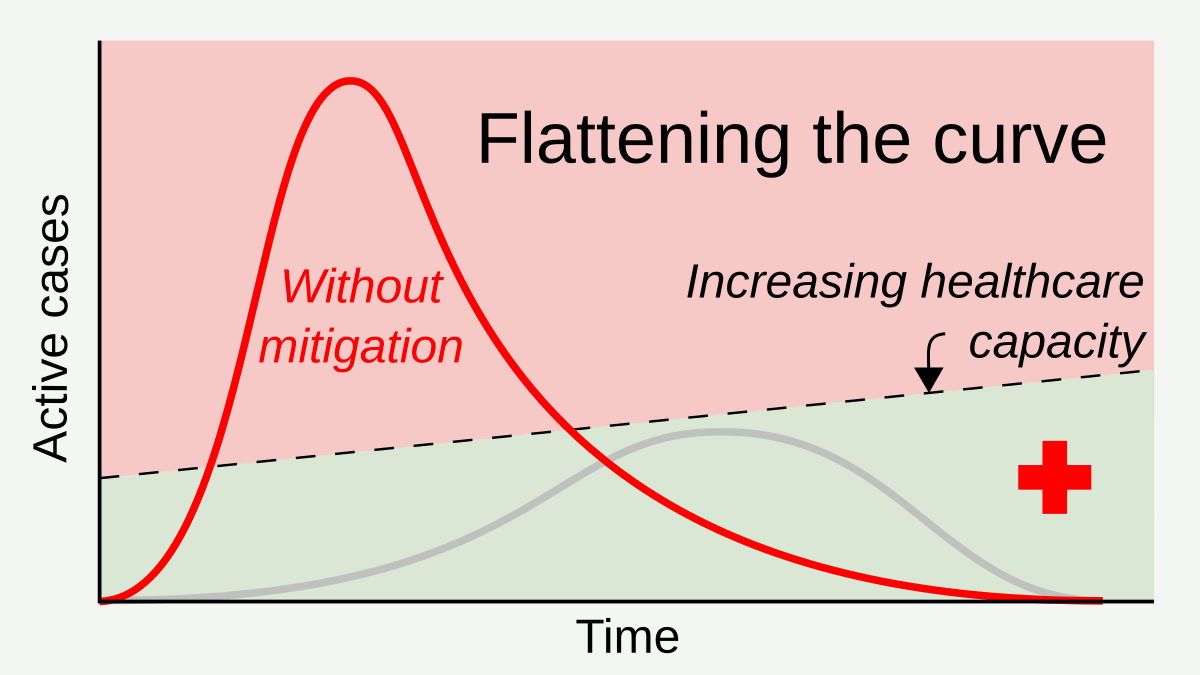
\includegraphics{exhibit/fig/flatten1.png}
\caption{RCraig09 2020}
\end{figure}
\end{frame}

\begin{frame}{Flattening the curve}
\protect\hypertarget{flattening-the-curve-1}{}
\begin{figure}
\centering
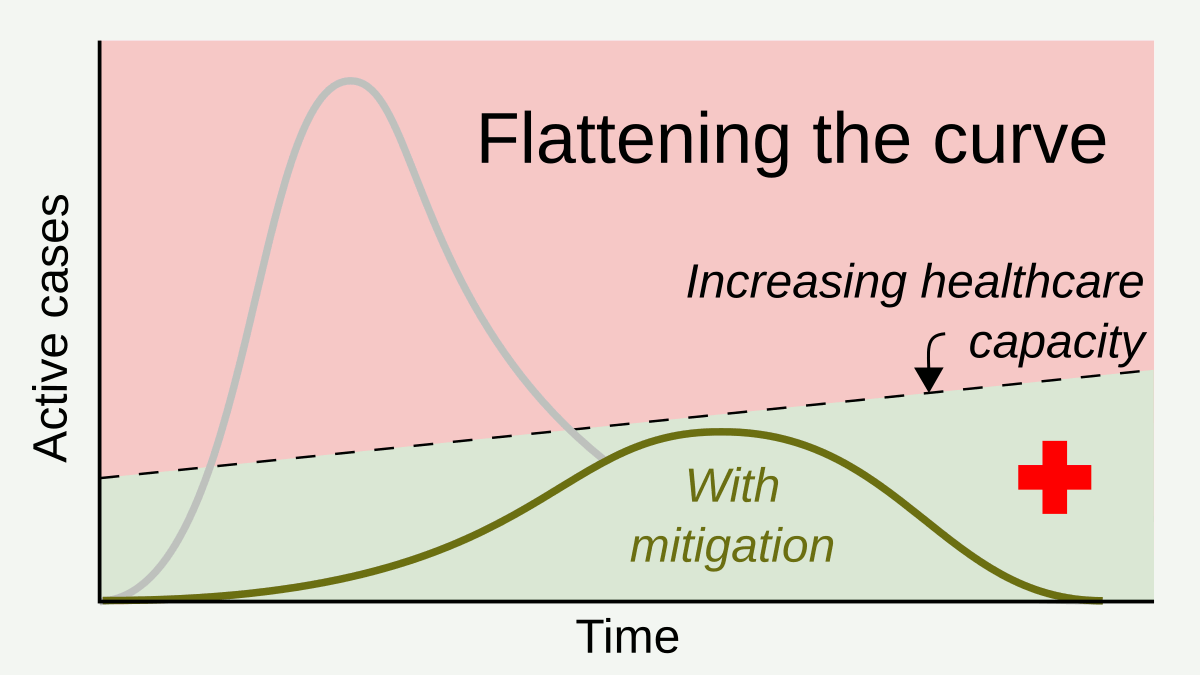
\includegraphics{exhibit/fig/flatten2.png}
\caption{RCraig09 2020}
\end{figure}
\end{frame}

\begin{frame}{People respond to incentives}
\protect\hypertarget{people-respond-to-incentives}{}
\begin{itemize}
\tightlist
\item
  Past data may lose its predictive power once people change their
  behavior (Lucas critique).

  \begin{itemize}
  \tightlist
  \item
    key missing element of SIR model
  \end{itemize}
\item
  There is voluntary social distancing, as well as non-compliance with
  policy measures.
\end{itemize}
\end{frame}

\begin{frame}{Systems matter}
\protect\hypertarget{systems-matter}{}
The SIR model is highly nonlinear. My getting sick depends on behavior
of others.

\begin{itemize}
\tightlist
\item
  difficult to forecast
\item
  externalities
\item
  non-intuitive
\end{itemize}
\end{frame}

\begin{frame}{Peaks of epidemics are notoriously hard to forecast}
\protect\hypertarget{peaks-of-epidemics-are-notoriously-hard-to-forecast}{}
\begin{figure}
\centering
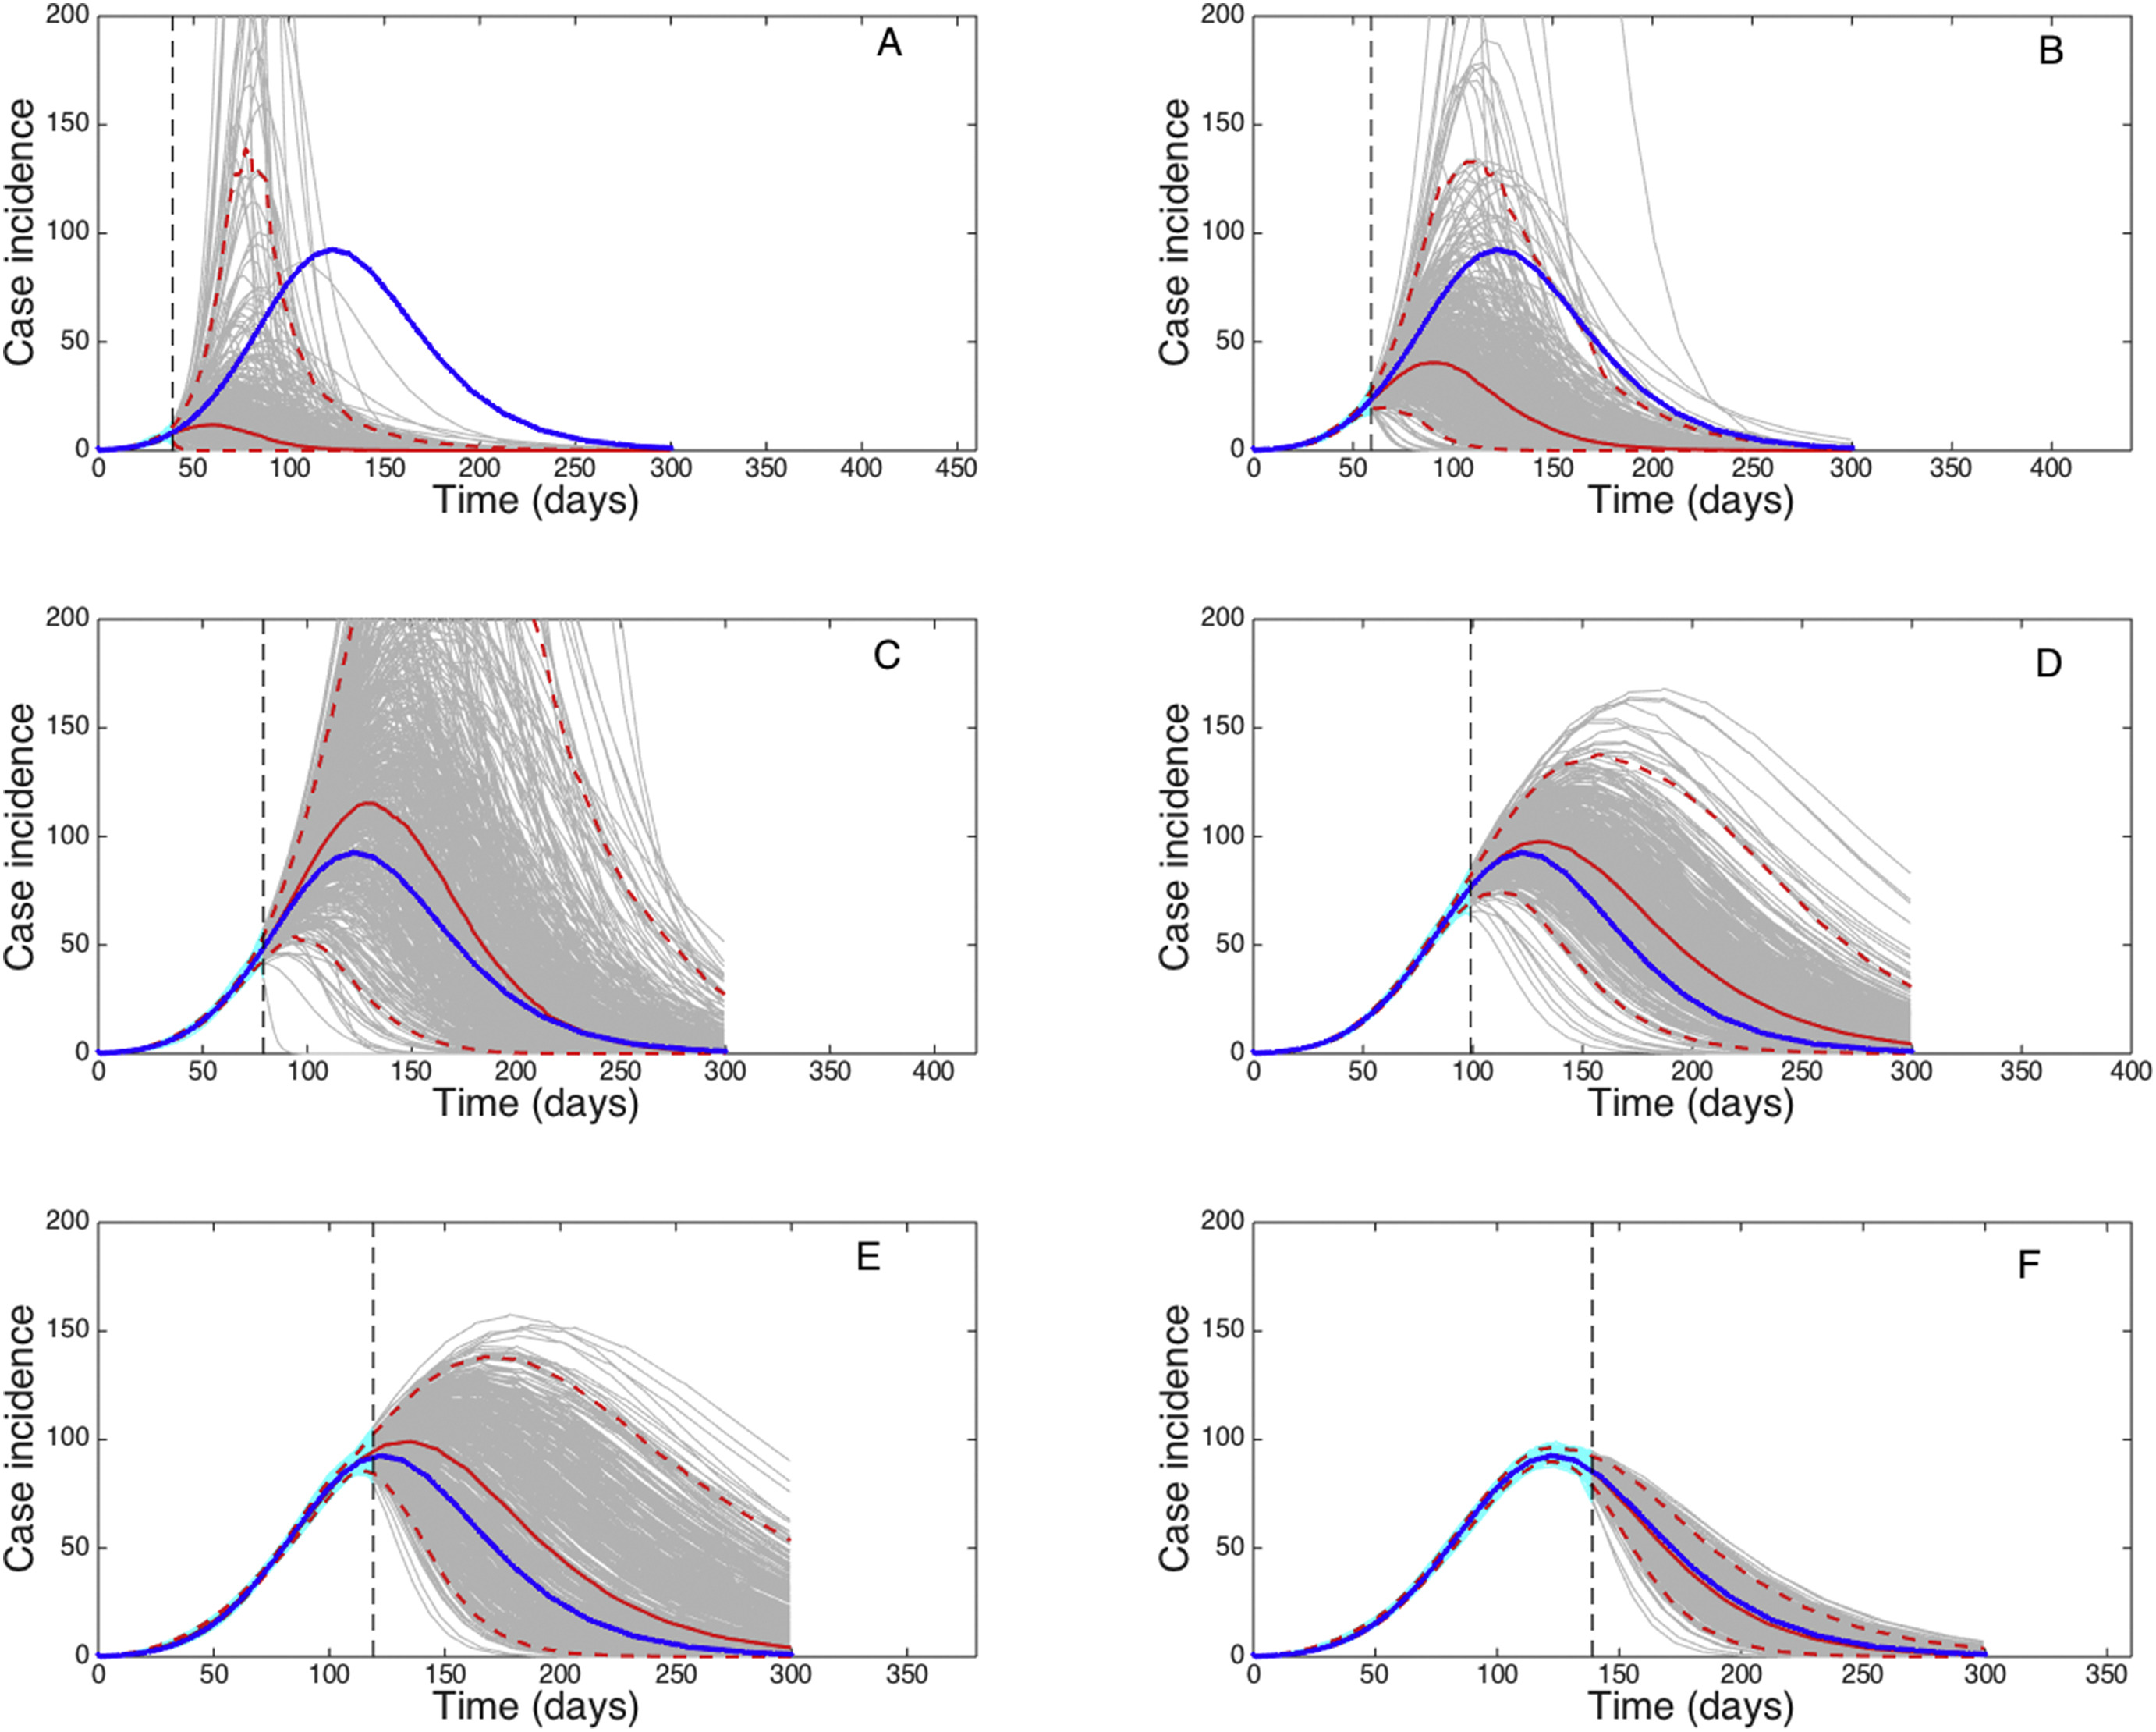
\includegraphics[width=\textwidth,height=0.8\textheight]{exhibit/fig/nonlinear.jpg}
\caption{Chowell 2017}
\end{figure}
\end{frame}

\begin{frame}{Lessons from economics}
\protect\hypertarget{lessons-from-economics}{}
\begin{itemize}
\tightlist
\item
  Even big data not sufficient to describe \emph{future} behavior.
  Understand incentives and externalities.
\item
  Hard to forecast non-linear system without theory.
\end{itemize}
\end{frame}

\hypertarget{conclusion-and-discussion}{%
\section{Conclusion and discussion}\label{conclusion-and-discussion}}

\begin{frame}{Conclusion and discussion}
\protect\hypertarget{conclusion-and-discussion-1}{}
\begin{enumerate}
\tightlist
\item
  Private sources of data can effectively \emph{complement} official
  statistics in times of urgency.
\item
  But \emph{rules} of statistics should always be followed.
\item
  Big data will never \emph{substitute} domain expertise, human
  judgement, ethical and political accountability.
\end{enumerate}
\end{frame}

\end{document}
